\documentclass[sigconf]{acmart}
\usepackage{booktabs}
\usepackage{graphicx}
\usepackage{xspace}
\usepackage{balance}
\emergencystretch=1em

\newcommand{\system}{AdAgentFlow-RT\xspace}

\title{AdAgentFlow-RT: A Contractual Runtime for Reliable High-Throughput Long-Horizon Multi-Agent Workflows}

\setcopyright{none}
\settopmatter{printacmref=false}
\acmConference[AAMAS '26]{Proceedings of the 25th International Conference on Autonomous Agents and Multiagent Systems}{May 25--29, 2026}{Paphos, Cyprus}
\acmYear{2026}
\copyrightyear{2026}
\acmDOI{}
\acmISBN{}
\renewcommand\footnotetextcopyrightpermission[1]{}

\author{Anonymous Authors}
\affiliation{\institution{Anonymous Institution}\country{}}

\begin{document}

\begin{abstract}
Existing agent benchmarks primarily measure whether an agent completes a task. This paper studies a complementary question: whether a long-horizon multi-agent runtime remains reliable, bounded, diagnosable, and recoverable under concurrent production-style execution. We present \system, a contractual runtime that represents workflows as contract-bearing execution graphs, monitors schema, semantic, dependency, resource, and recovery contracts, localizes faults, applies bounded recovery, and records event-sourced traces. We do not introduce a new task dataset. Instead, we build a production-stress evaluation harness on top of public workloads from tau2-bench / tau3-bench and AgentChangeBench. The harness preserves benchmark-native metrics while adding runtime stability metrics such as dead-letter rate, recovery success, retry amplification, silent failure rate, fault propagation depth, contaminated artifact count, and mean time to detect and recover. In the LLM-backed evaluation, vanilla tool calling silently succeeds on a large fraction of runs and incurs the highest cost per successful task (7.40), while the full runtime is the only configuration that achieves zero silent failures, the lowest dead-letter rate (0.41), and a non-zero recovery success rate (0.40). The artifact includes the runtime kernel, the production-stress harness, four runtime strategies, seven stressors, full ablations, JSONL traces, aggregated summaries, and the LaTeX draft.

\end{abstract}

\begin{CCSXML}
<ccs2012>
 <concept>
  <concept_id>10010147.10010178.10010179</concept_id>
  <concept_desc>Computing methodologies~Multi-agent systems</concept_desc>
  <concept_significance>500</concept_significance>
 </concept>
 <concept>
  <concept_id>10011007.10011006.10011041</concept_id>
  <concept_desc>Software and its engineering~Runtime environments</concept_desc>
  <concept_significance>300</concept_significance>
 </concept>
</ccs2012>
\end{CCSXML}

\ccsdesc[500]{Computing methodologies~Multi-agent systems}
\ccsdesc[300]{Software and its engineering~Runtime environments}
\keywords{multi-agent systems, runtime reliability, fault injection, runtime verification, agent benchmarks}

\maketitle

\section{Introduction}

Long-horizon agent systems increasingly combine planning, tool use, memory, verification, and multiple specialized agents. Public benchmarks have improved the field's ability to measure task completion, but production deployments face a broader reliability problem: the runtime must bound cost, detect contract violations, avoid silent failures, contain faulty artifacts, recover without unbounded retry loops, and preserve traces that support diagnosis.

\system reframes an existing multi-agent engineering prototype as a contractual runtime for reliable high-throughput multi-agent workflows. The prior advertising generation workflow remains an example domain plugin. The paper contribution is a reusable runtime abstraction and a stress evaluation harness that can wrap public task environments without changing their task data.

This work studies three research questions. First, can executable contracts over schemas, semantics, dependencies, budgets, and recovery policies turn malformed or off-policy agent outputs into explicit runtime events rather than implicit downstream corruption? Second, can bounded recovery avoid the retry amplification of retry-only execution while preserving a non-zero recovery path under injected production faults? Third, can event-sourced traces make runtime failures auditable enough to support fault localization and reproducible post-hoc diagnosis?

The main matrix is run against the live Qwen3-8B endpoint served by vLLM 0.23.0 and the public \mbox{$\tau^3$}-bench and AgentChangeBench task fixtures. The evidence does not support a simple ``highest task-success'' claim: schema-only validation slightly outperforms the full runtime on raw \mbox{$\tau^3$}-bench task success (15.3\% vs.\ 14.8\%). Instead, the current result supports a narrower runtime claim: \system{} is the only evaluated configuration with non-zero bounded recovery on the main matrix, while retry-only amplifies calls without producing runtime-level diagnosis. Across 1{,}392 live-LLM rows, all four configurations report zero measured silent failures; we therefore treat silent-failure reduction as a metric definition and audit signal, not as standalone evidence that contracts are sufficient.

The key distinction from a benchmark paper is that the workload is not new. tau2-bench / \mbox{$\tau^3$}-bench and AgentChangeBench provide public task environments and fixture metadata~\cite{tau2bench,agentchangebench}. \system contributes the execution substrate around those tasks: contract enforcement, fault localization, bounded recovery, dead-letter handling, and trace-derived reliability metrics.

This paper makes the following contributions:

\begin{itemize}
    \item A contractual execution graph for long-horizon multi-agent workflows, including contracts over artifacts, dependencies, resources, and recovery behavior.
    \item Executable contracts and bounded recovery semantics implemented in a runtime kernel with a scheduler, monitor, artifact store, fault localizer, recovery controller, and event-sourced trace.
    \item A production-stress harness that reuses public benchmark fixtures while running comparable runtime strategies under matched models, tools, fault distributions, concurrency, and recovery budgets.
    \item A trace-derived reliability metric suite that complements fixture-backed task success with dead-letter rate, recovery success, retry amplification, explicit contract violations, and auditability signals.
\end{itemize}

The current artifact includes deterministic smoke tests for development and an audited external main matrix for tau2-bench / \mbox{$\tau^3$}-bench and AgentChangeBench. The paper claims in Section~\ref{sec:experiments} are generated from the external matrix rather than smoke rows.

\section{Background and Motivation}

Multi-agent workflows fail in ways that are not captured by final task success alone. A workflow can complete while using stale context, propagating a contaminated artifact, violating a resource budget, silently accepting a malformed tool response, or retrying until cost becomes unacceptable.

Retry and prompt repair are useful but insufficient as the only reliability mechanism. They do not identify the responsible node, downstream contamination, recovery budget, or whether the runtime should rollback, reroute, degrade, escalate, or dead-letter a task.

\section{Contractual Execution Model}
\label{sec:method}

\system models a multi-agent workflow as a Contractual Execution Graph. Nodes declare a role, capability, agent provider, and contract name. Edges declare artifact dependencies. Contracts define input and output schemas, preconditions, postconditions, semantic checks, resource budgets, recovery policies, and escalation policies.

The first implementation supports DAG execution, including sequential paths, fan-out, joins, fallback branches, and rollback targets. Each produced artifact carries provenance, validation status, and downstream consumers. This makes failure propagation explicit and measurable.

\subsection{Contracts}

A contract binds a runtime capability to observable obligations:

\begin{itemize}
    \item \textbf{Schema contract}: validates inputs and outputs.
    \item \textbf{Semantic contract}: captures domain invariants such as policy compliance or goal alignment.
    \item \textbf{Dependency contract}: requires upstream artifacts to exist and be valid before a node runs.
    \item \textbf{Budget contract}: bounds latency, LLM calls, tool calls, tokens, and retries.
    \item \textbf{Recovery contract}: lists permitted recovery actions and escalation behavior.
\end{itemize}

The current implementation represents contracts as typed Python dataclasses and supports JSON-Schema validation with a dependency-light fallback validator for minimal environments.

\subsection{Artifacts and Propagation}

Every node produces zero or more artifacts. An artifact records its producer, contract name, content, validation status, provenance, and downstream consumers. When a contract violation occurs, the runtime localizes the responsible node and traverses the graph to estimate affected downstream nodes and contaminated artifacts. These quantities directly support the metrics \textit{fault propagation depth} and \textit{contaminated artifact count}.

\subsection{Bounded Recovery}

Recovery is selected from a bounded policy rather than an open-ended retry loop. The controller currently supports quick repair, retry, mock reroute, rollback target selection, downstream invalidation, degradation, human escalation, and dead-letter. A recovery decision records the selected action, target node, reason, budget cost, and whether execution may continue.

\section{\system Runtime}
\label{sec:system}

The runtime contains a contract registry, scheduler, monitor, artifact store, fault localizer, recovery controller, event log, and replay utilities. Before a node runs, the monitor checks dependency and precondition contracts. After execution, it checks schema and budget contracts and emits violations. The fault localizer maps violations into operational classes such as artifact, coordination, resource, tool-environment, runtime, and verifier faults. The recovery controller selects bounded actions such as quick repair, retry, reroute, rollback, invalidation, degradation, human escalation, or dead-letter.

Every event is traceable by task identifier and run identifier. Events include graph creation, contract checks, node scheduling, artifact production, violations, fault diagnoses, recovery decisions, checkpoints, rollbacks, dead letters, and task finalization.

\begin{figure}[t]
    \centering
    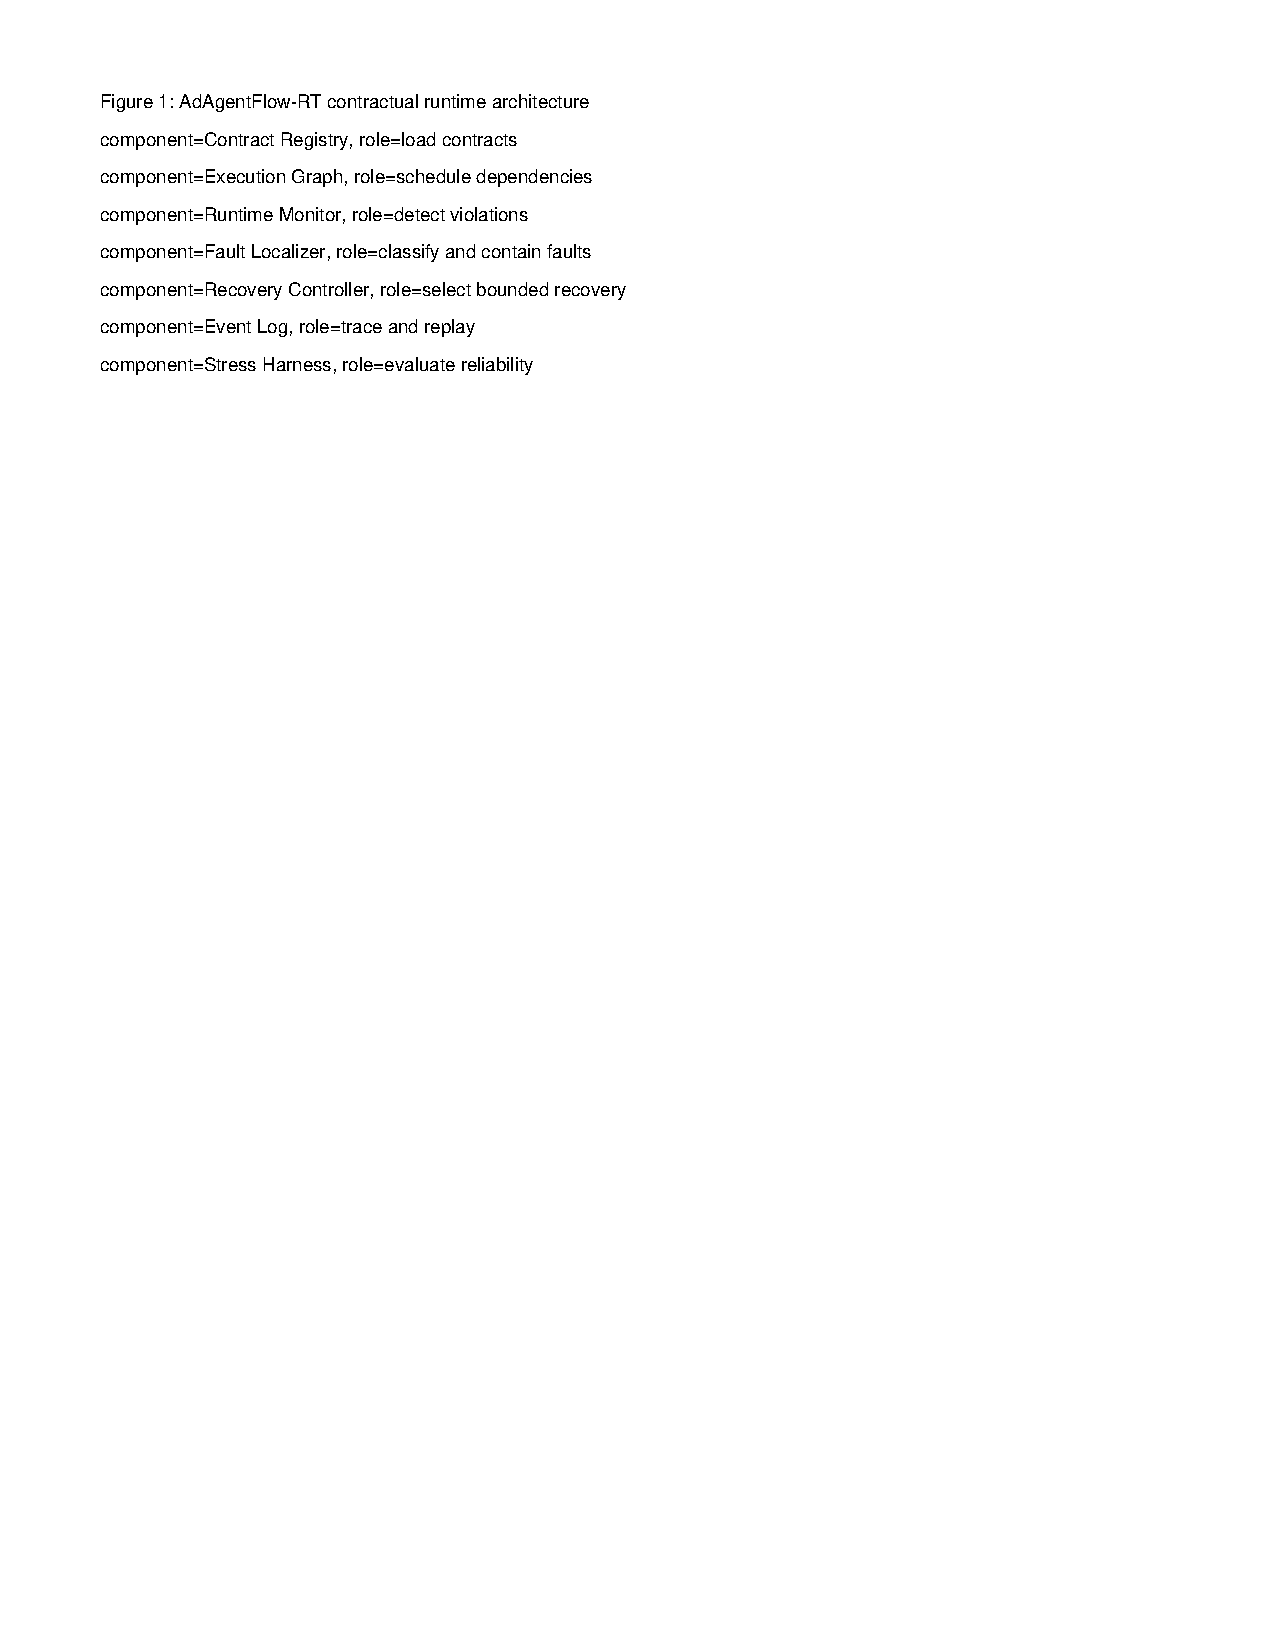
\includegraphics[width=\linewidth]{figs/system_architecture.pdf}
    \Description{A component diagram listing the contract registry, execution graph, runtime monitor, fault localizer, recovery controller, event log, and stress harness.}
    \caption{\system contractual runtime components.}
    \label{fig:system}
\end{figure}

\subsection{Runtime Kernel}

Figure~\ref{fig:system} shows the runtime components. The contract registry stores executable contract specifications. The graph planner constructs a dependency graph. The scheduler selects runnable nodes whose dependencies are satisfied. The monitor checks contracts before and after node execution. The artifact store records produced artifacts and validation status. The fault localizer maps violations into operational fault classes. The recovery controller selects bounded actions from policy and remaining budget. The event log records each runtime transition for replay and metric extraction.

\subsection{Event-Sourced Trace}

The event log records `graph.created', `contract.loaded', `node.started', `contract.checked', `fault.injected', `contract.violated', `fault.localized', `recovery.started', `recovery.selected', `recovery.succeeded', `artifact.produced', `dead\_letter.created', and `task.finalized'. Each event carries `task\_id', `run\_id', optional `node\_id', status, payload, and timestamp. The smoke harness also records relative millisecond offsets so trace metrics can estimate mean time to detect and recover.

\subsection{Runtime Strategies}

The harness implements four comparable strategies:

\begin{itemize}
    \item \textbf{Vanilla}: directly executes the benchmark-style task without runtime contracts or recovery.
    \item \textbf{Retry-only}: retries after failure until a bounded retry count is exhausted.
    \item \textbf{Schema-only}: validates schema and applies repair/retry, but does not localize graph-level faults.
    \item \textbf{\system}: applies contract monitoring, fault localization, bounded recovery, artifact invalidation hooks, dead-letter handling, and event trace.
\end{itemize}

\section{Production-Stress Evaluation Harness}

The harness wraps public benchmark tasks without modifying their data. tau2-bench / tau3-bench provide the main workload across airline, retail, and telecom domains. AgentChangeBench provides supplementary goal-change recovery evaluation across airline and retail domains.

We compare vanilla tool calling, retry-only execution, schema-only validation, and AdAgentFlow-RT. Stressors include tool timeouts, rate limits, partial responses, schema drift, stale context, duplicate messages, and worker crashes. All experiments write JSONL records with benchmark-native metrics, runtime metrics, injected faults, events, and recovery outcomes.

\section{Experiments}

The smoke setting runs three tasks per domain, one trial, concurrency one, no injected faults, and all four runtime methods. The main setting varies concurrency, fault rate, domains, trials, and runtime strategy.

Planned figures include success rate versus concurrency, latency versus concurrency, recovery and dead-letter rate versus fault rate, cost per successful task, AgentChangeBench recovery metrics, and ablation results. Planned tables include framework comparisons, tau3 results, runtime stability metrics, ablations, and recovery action distributions.

\section{Discussion}

The contractual runtime trades additional monitoring and trace overhead for improved diagnosability and bounded recovery. The key limitation is that semantic checks require domain-specific verifiers or benchmark-specific policies. The harness is designed so stronger verifiers can be added without changing workload data.

\subsection{Cost and Reliability}

Contracts and traces add runtime work. The relevant tradeoff is not raw latency alone, but cost per successful task under fault injection. A retry-only strategy may appear simple, but can amplify tool and LLM calls without identifying the contaminated artifact. \system pays monitoring overhead to make violations and recovery decisions inspectable. In the current main matrix, schema-only slightly leads raw task success, while the full runtime is the only configuration with non-zero bounded recovery and lower cost per successful task than retry-only. This is a failure-containment claim, not a task-success leaderboard claim.

\subsection{Limits of the Current Artifact}

The current artifact is external-benchmark backed: all four runtime methods are driven by the \texttt{SyncLLMClient} against public benchmark task fixtures, and the main matrix is gated by an audit script that requires both external main-matrix rows and AgentChangeBench rows. The harness still includes deterministic smoke modes for development and regression tests, but those rows are not used for the paper's main claims. The remaining limitations are important: the scorer is fixture-backed rather than a full benchmark-native simulator rerun; the matrix uses a single Qwen3-8B endpoint; and several trace metrics such as mean time to detect, mean time to recover, fault propagation depth, and contaminated artifact count are placeholders unless timestamped traces and artifact-propagation annotations are present. These limits motivate a controlled successful-trajectory fault-injection study as the next experiment.

\subsection{Threats to Validity}

Fault distributions may not match all production incidents. Semantic contracts can be incomplete or domain-biased. The task fixtures are public and external, but the execution uses one live LLM endpoint and a constrained sampling plan; stronger production claims require benchmark-native simulator reruns, additional models, larger task sweeps, independent reruns, and controlled fault injection on trajectories that first succeed without injected faults. These limits affect generality, not the artifact's audit trail: the JSONL traces, summary tables, figures, and audit report are all generated from the same external main-matrix directory.

\section{Related Work}

This work relates to agent benchmarks, multi-agent frameworks, runtime verification, workflow orchestration, fault injection, chaos engineering, and production observability. Unlike task-only benchmark evaluations, AdAgentFlow-RT focuses on operational reliability under stress.

\section{Conclusion}

\system evaluates and improves the runtime reliability of long-horizon multi-agent workflows. Rather than introducing a new dataset, it layers production stress, contractual monitoring, fault localization, bounded recovery, and event-sourced tracing on top of public benchmark task fixtures. The current artifact establishes the runtime kernel, stress harness, baselines, stressors, trace-derived metrics, ablations, external main-matrix results, publication-facing figures, paper tables, and audit gate. The next step is not to create more infrastructure, but to harden the paper for submission: broaden model coverage where time permits, polish the plots and prose, and package a clean reproducibility artifact.


\begin{acks}
The authors thank the maintainers of \mbox{$\tau^3$}-bench and AgentChangeBench for the public task environments that motivate the production-stress evaluation harness in this paper. The main-matrix evidence was produced with a live Qwen3-8B endpoint served by vLLM 0.23.0 and audited from the external result directory. The artifact includes JSONL traces, summary tables, regenerated figures, and an audit report; full reproduction instructions are provided in the runbook.
\end{acks}

\bibliographystyle{ACM-Reference-Format}
\bibliography{refs}

\end{document}
